\aufgabe[6]
Der Verkettungsfaktor $k$ gibt in Mehrphasensystemen das Verhältnis der elektrischen Spannung zwischen zwei benachbarten Außenleitern zum Wert der Sternspannung zwischen einem beliebigen Außenleiter und dem Sternpunkt an.

Leiten Sie formelmäßig den Verkettungsfaktor $k = |\underline{U_{12}}|/|\underline{U_{10}}|$ eines $m$-phasigen Wechselstromnetzes an Hand der von Ihnen zu vervollständigenden Skizze her!

\vskip 12pt
\begin{center}
	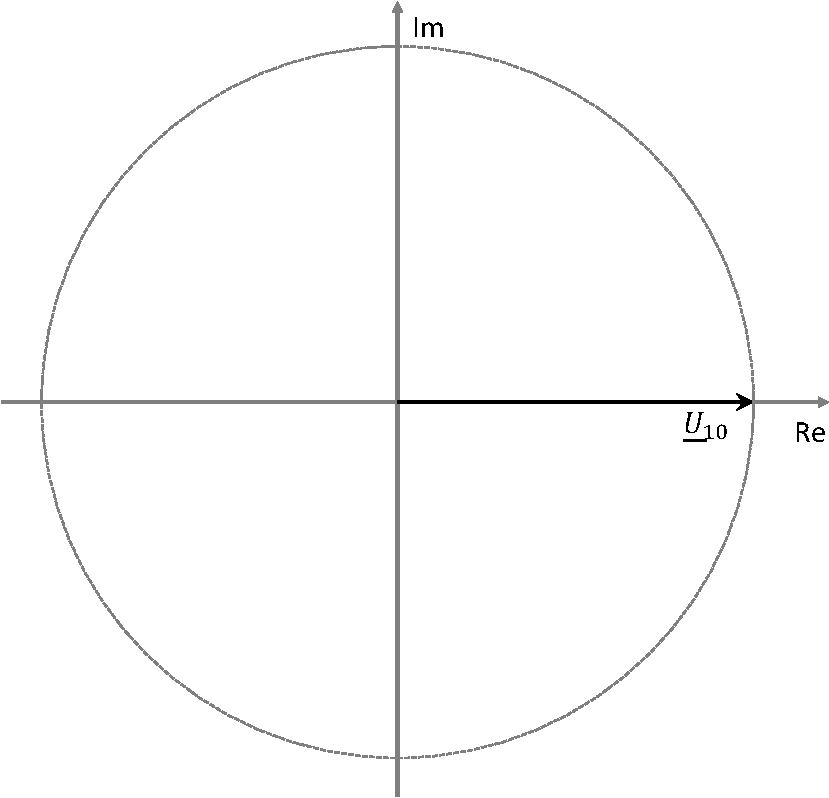
\includegraphics[width=13cm]{aufgabe_xyz/aufgabe4-crop}
\end{center}

\begin{solution}[15cm]
	\begin{center}
		\[ k = |\underline{U_{12}}|/|\underline{U_{10}}| = 2 \cdot \sin \left(\frac{\mathrm{\pi}}{m} \right)\]
	\end{center}
\end{solution}

\newpage